
\section{Implementation}
\label{Implementation}

In diesem Kapitel wird die Implementation der einzelnen Container beschrieben, wie sie im Kapitel \ref{Architektur:Container} definiert wurden.

\subsection{ÖV-Güteklassen 2018 Generator}
\label{Implementation:ÖV-Güteklassen 2018 Generator}

\subsubsection{Datenaufbereitung}
\label{ÖV-Güteklassen 2018 Generator:Datenaufbereitung}

Der \acs{ÖV}-Güteklassen 2018 Generator operiert auf unterschiedlichen Daten von externen Datenquellen.
Diese Daten kommen in den verschiedensten Formaten daher und müssen für eine weitere Verarbeitung gefiltert, aufbereitet und optimiert werden.
Für eine einfache Handhabung wurde ein Docker-Setup gewählt.
Die Bedienung dieses Setups ist im Kapitel \ref{Softwaredokumentation} ausführlich beschrieben.

Grundsätzlich kann man sagen, dass zwei Docker-Container existieren, namentlich \emph{tooling} und \emph{db}.
Der Docker-Container \emph{tooling} nimmt Daten entgegen oder bezieht diese von externen Diensten und bereitet sie so vor, dass diese vom Docker-Container \emph{db} in die Datenbank \emph{oevgk18} für eine Weitereverwendung des \acs{ÖV}-Güteklassen 2018 Generators geladen werden können.
Der Docker-Container \emph{db} sorgt ebenfalls dafür, dass beim Starten die nötigen Extensions (pgrouting, hstore, \dots) aktiviert sind und zuerst die Schemas und danach die Stored Procedures erstellt werden.
Zusätzlich müssen nach den einzelnen Imports, welche nachfolgend beschrieben werden, zusätzliche Modifaktionen am Schema vorgenommen werden.
Diese Modifikationen werden in einem Post-Import-Schritt durchgeführt, weil die Terrain- sowie die OSM-Daten durch Tools importiert werden, welche ein Schema vorgeben und somit bereits vorhandene Schemas überschrieben werden.
Ebenfalls werden zusätzliche Indizes erstellt.

Im weiteren sind die Services, welche die beiden Docker-Container bereitstellen, anhand eines Datenflussdiagramms aufgeschlüsselt.
Der \acs{ÖV}-Güteklassen 2018 Generator operiert grundsätzlich auf drei externen Datenquellen, namentlich sind das die Fahrplandaten (nachfolgend \emph{gtfs data}), das Terrainmodell (nachfolgend \emph{terrain data)} und die \acs{OSM}-Daten (nachfolgend \emph{osm data}).
Für jede Datenquelle existiert ein Service im Docker-Container \emph{tooling} und ein Pendant im Docker-Container \emph{db}, welche die vorverarbeiteten Daten des Docker-Containers \emph{tooling} entgegennimmt und in die Datenbank spielt.

\paragraph{OSM-Daten}~\\
\acs{OSM}-Daten werden von der Routing-Engine für das Berechnen von \glspl{Isochrone} und für das Identifizieren von \acs{ÖV}-Haltestellen verwendet.
In Abbildung \ref{fig:dataflow-docker-setup-osm-data} ist ersichtlich, wie der Docker-Container \emph{tooling} die \acs{PBF}-Datei der Schweiz von einem externen Dienst~\cite{planet_osm_ch} bezieht und für die zwei vorhin erwähnten Zwecke vorbereitet.
Es besteht ebenfalls die Möglichkeit, eine lokale \acs{OSM}-Datei zu verwenden.
Dies ist vorallem für Testing-Zwecke vorteilhaft, da auf kleineren Ausschnitten leichter getestet werden kann.

\begin{figure}[ht]
    \centering
    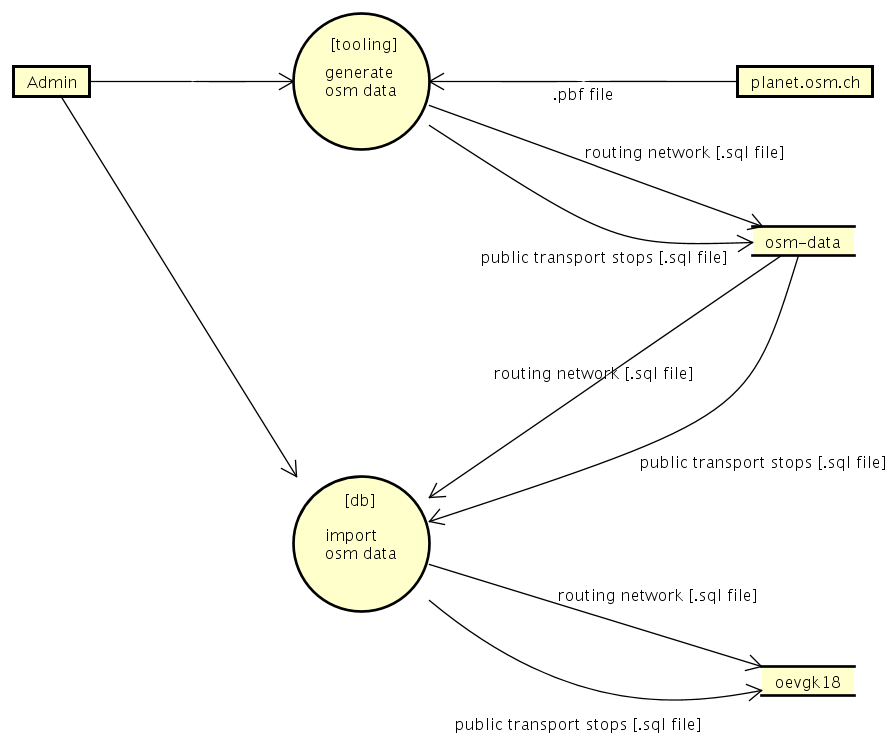
\includegraphics[width=0.8\linewidth]{projectdoc/img/dataflow-docker-setup-osm-data.png}
    \caption[Datenfluss Setup OSM-Daten]{Datenfluss Setup OSM-Daten}
    \label{fig:dataflow-docker-setup-osm-data}
\end{figure}

Der Routing-Graph wird mithilfe des Tools \emph{OSM2PO}~\cite{OSM2PO} für pgRouting aufbereitet und als SQL-Datei bereitgestellt.
\emph{OSM2PO} wird durch eine separate Konfiguration für unsere Zwecke konfiguriert, so dass die Routen für Fussgänger optimiert werden.

\paragraph{GTFS-Daten}~\\
Die Fahrplandaten werden im Docker-Container \emph{tooling} automatisch von geOps~\cite{geops_fahrplandaten} im GTFS-Format~\cite{gtfs_spec} heruntergeladen und im CSV-Format als TXT-Dateien bereitgestellt.
Diese wiederum können in einem nächsten Schritt durch den Docker-Container \emph{db} in die Datenbank gespielt werden.
Der Datenfluss ist in Abbildung \ref{fig:dataflow-docker-setup-gtfs-data} ersichtlich.

\begin{figure}[ht]
    \centering
    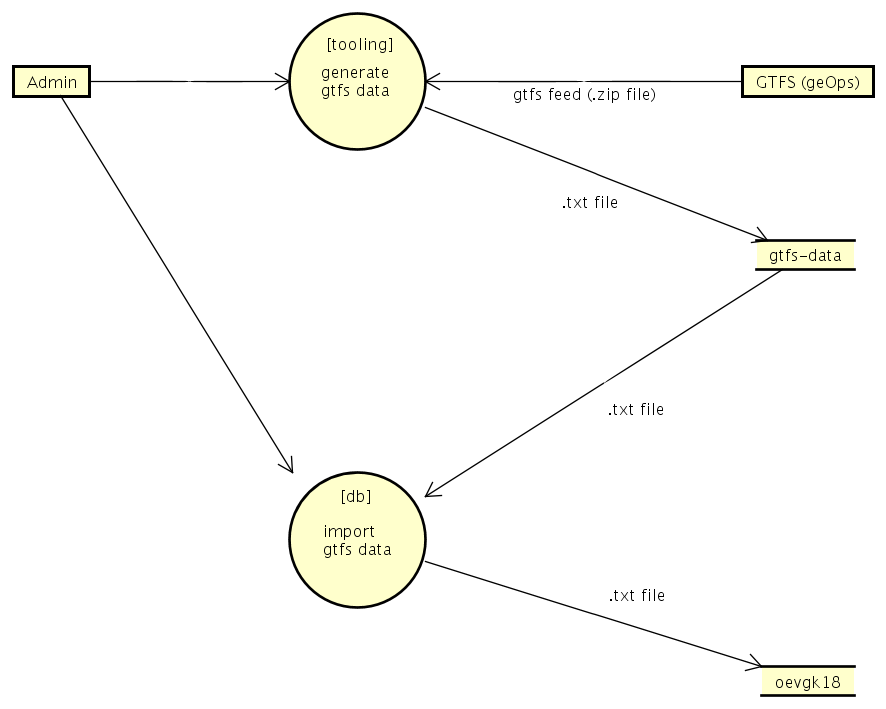
\includegraphics[width=0.8\linewidth]{projectdoc/img/dataflow-docker-setup-gtfs-data.png}
    \caption[Datenfluss Setup GTFS-Daten]{Datenfluss Setup GTFS-Daten}
    \label{fig:dataflow-docker-setup-gtfs-data}
\end{figure}

\paragraph{Terrain-Daten}~\\
Das Terrainmodell kann aufgrund der Grösse der Datei und aus lizenztechnischen Gründen nicht von einem externen Dienst bezogen und muss somit dem Service manuell als TIF-Datei bereitgestellt werden.
Diese Datei wird mit raster2pgsql~\cite{raster2pgsql} verarbeitet, einem Tool von PostGIS, welches Raster-Formate in ein Format konvertiert, welches in eine PostGIS-Tabelle geladen werden kann.
Dabei wird von der üblichen Struktur (ein Service im Docker-Container \emph{tooling} und ein Pendant im \emph{db}) abgewichen.
raster2pgsql ist darauf ausgelegt, direkt in eine PostgreSQL-Datenbank zu schreiben.
Der Weg über eine Intermediate-Datei wäre somit eine überflüssige Indirektion.
Somit entfällt hier der Service im Docker-Container \emph{tooling}.
Der Datenfluss ist in Abbildung \ref{fig:dataflow-docker-setup-terrain-data} ersichtlich.

\begin{figure}[ht]
    \centering
    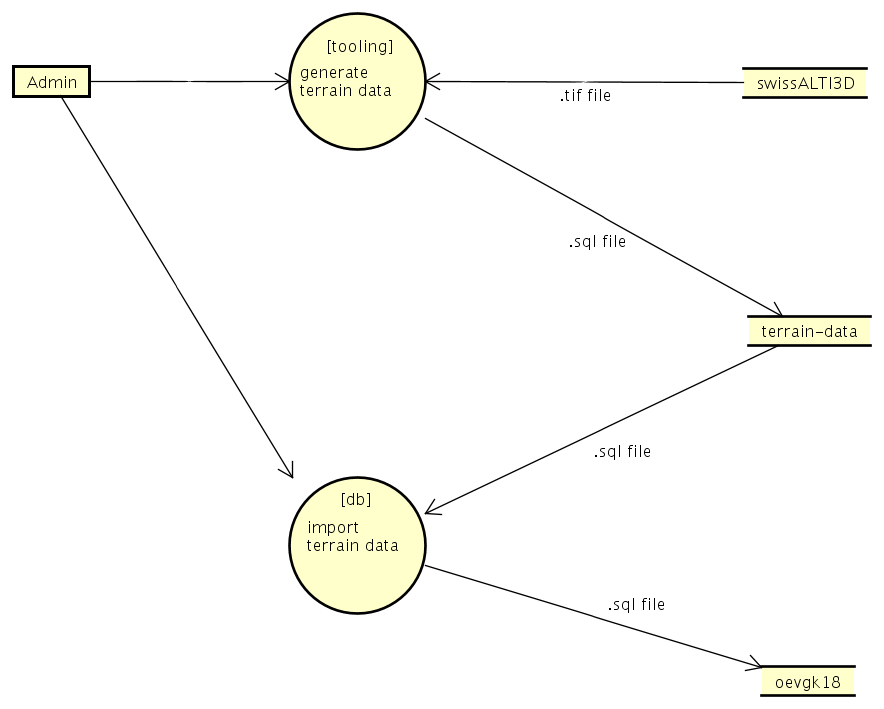
\includegraphics[width=0.8\linewidth]{projectdoc/img/dataflow-docker-setup-terrain-data.png}
    \caption[Datenfluss Setup Terrain-Daten]{Datenfluss Setup Terrain-Daten}
    \label{fig:dataflow-docker-setup-terrain-data}
\end{figure}

\subsubsection{Umsetzung Spezifikation}
\label{ÖV-Güteklassen 2018 Generator:Umsetzung Spezifikation}

\paragraph{Datenfluss}~\\
Durch die unterschiedliche Natur der Datenquellen und der Menge dieser ist es hilfreich, zu visualisieren, zu welchem Zeitpunkt welche Daten zu welchem Zweck benötigt werden.
Wie in Abbildung \ref{fig:Flow_OeVGK_Brechnung} ersichtlich ist, werden die \acs{ÖV}-Güteklassen in fünf Schritten berechnet. 
In Abbildung \ref{fig:dataflow_OeV-Gueteklassen_2018_Generator} ist nun schematisch die Raison d’Être der Datenquellen ersichtlich.
Die Pfeilrichtung beschreibt den Datenfluss.

\begin{figure}[ht]
    \centering
    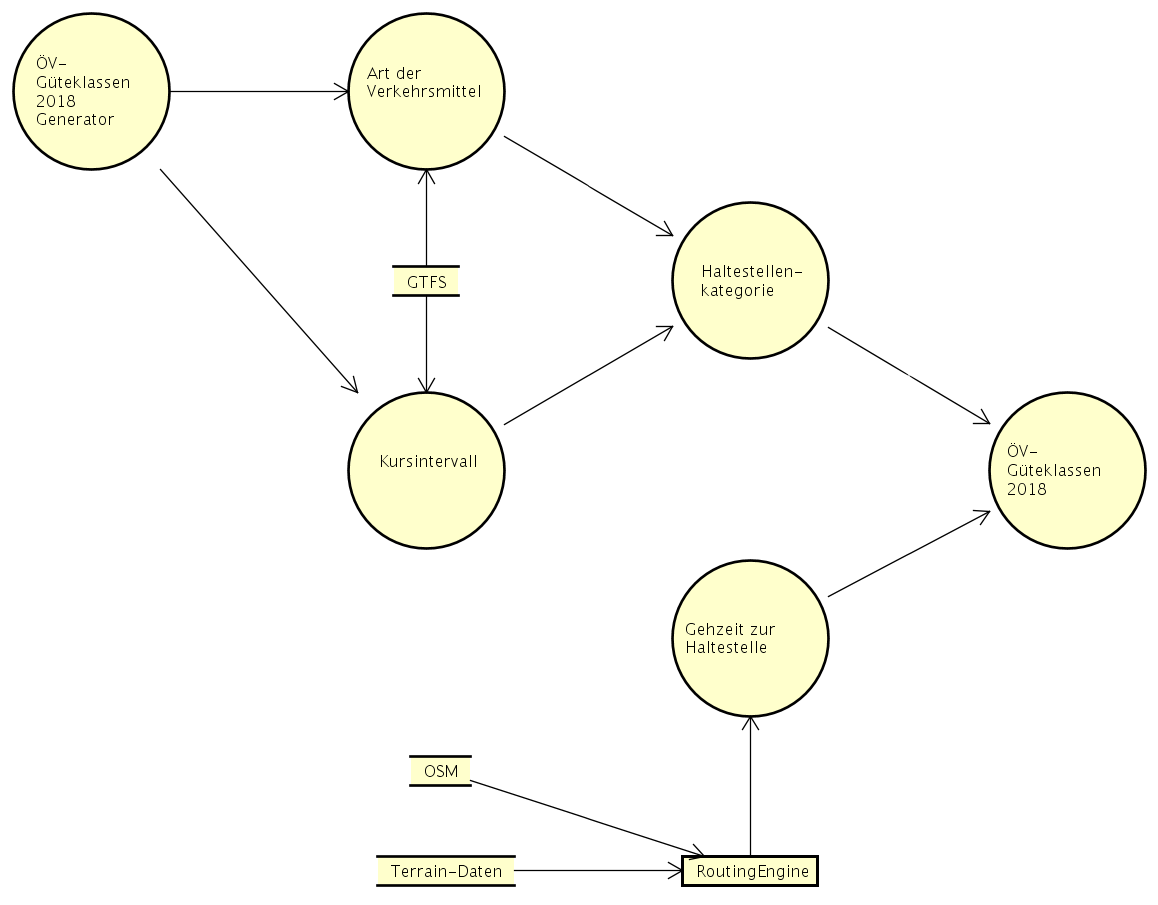
\includegraphics[width=1.0\linewidth]{projectdoc/img/dataflow_OeV-Gueteklassen_2018_Generator.png}
    \caption[Datenfluss ÖV-Güteklassen 2018 Generator]{Datenfluss ÖV-Güteklassen 2018 Generator}
    \label{fig:dataflow_OeV-Gueteklassen_2018_Generator}
\end{figure}

Die Datenquellen \emph{GTFS}, \emph{OSM} und \emph{Terrain-Daten} entsprechen an sich keinen separaten Datenquellen, sondern werden nur zum besseren Verständnis getrennt dargestellt.
Wie wir in Kapitel \ref{ÖV-Güteklassen 2018 Generator:Datenaufbereitung} gesehen haben, werden diese aufbereitet und in einer Datenbank \emph{oevgk18} gehalten.

Nachfolgend werden die fünf Berechnungsschritte separat beschrieben.

\paragraph{Berechnung der Art der Verkehsmittel}~\\
Die öffentlichen Verkehrsmittel werden in drei Verkehrsmittelgruppen gruppiert (siehe Kapitel \ref{Berechnungsmethodik OeVGK18:Art der Verkehrsmittel} im Teil \ref{Technischer Bericht}).
Wie in Kapitel \ref{subsystem:GTFS} beschrieben werden die Fahrplandaten im \acs{GTFS}-Format~\cite{gtfs_spec} gehalten. 
Es werden dabei 8 Verkehrsmittel-Typen unterschieden.
In Tabelle \ref{table:Mapping GTFS Route Type Verkehrsmittelgruppe} ist ein Mapping der definierten GTFS Route Typen zu den Verkehrsmittelgruppen ersichtlich.

\begin{table}[ht]
    \centering
    \begin{tabular}[ht]{l l}
        \toprule
        \textbf{GTFS Route Type} 
                                & \textbf{Verkehrsmittelgruppe}\\
        \midrule
        0 (Tram, Streetcar, Light rail)
                                & C\\
        1 (Subway, Metro)
                                & A/B\\
        2 (Rail)
                                & A/B\\
        3 (Bus)
                                & C\\
        4 (Ferry)
                                & C\\
        5 (Cable car)
                                & C\\
        6 (Gondola, Suspended cable car)
                                & C\\
        7 (Funicular)
                                & C\\            
        \bottomrule
    \end{tabular}
    \caption{Mapping GTFS Route Type Verkehrsmittelgruppe}
    \label{table:Mapping GTFS Route Type Verkehrsmittelgruppe}
\end{table}

Die Herausforderung beim Berechnen der Art der Verkehrsmittel ist die Bestimmung der Bahnknoten.
Die Definition des Bahnknoten ist im Kapitel \ref{Berechnungsmethodik OeVGK18:Art der Verkehrsmittel} genau spezifiziert.
Für die Klassifizierung eines Bahnknoten ist die Anzahl der Richtungen, in welche man von einer Bahnstation aus verkehren kann, relevant.

\begin{listing}[ht]
    \inputminted{sql}{projectdoc/listing/count_of_distinct_next_stops.sql}
    \caption{SQL-Query zur Bestimmung der Anzahl erreichbaren Haltestellen (finale Version)}
    \label{listing:count_of_distinct_next_stops}
\end{listing}

In Listing \ref{listing:count_of_distinct_next_stops} ist ersichtlich, wie für eine spezifizierte Auswahl an Haltestellen (\emph{relevant\_stops}) die Anzahl erreichbaren Haltestellen gezählt wird.
Im abgebildeten Query wird geprüft, ob der aktuelle Stop bei einem anderen \emph{Trip} als vorherige Haltestelle vorkommt.
Die Anzahl wird mit der Window Function gesammelt und gruppiert für jede Haltestelle retourniert.

Die abgebildete Berechnung hat mehrere Ver- und Verschlimmbesserungen durchlaufen.
Es lohnt sich einen ausführlicheren Blick auf die Evolution der Abfragetechnik zu legen, da diese Hoch und Tiefs durchlebt hat und einige Erkenntnisse daraus gezogen wurden.

\subparagraph{1. Version}
In einer ersten Version war angedacht, dass das Berechnen der Anzahl erreichbaren Haltestellen für jede einzelne Haltestelle separat aufgerufen wird.

\begin{listing}[ht]
    \inputminted{sql}{projectdoc/listing/count_of_distinct_next_stops_v1.sql}
    \caption{SQL-Query zur Bestimmung der Anzahl erreichbaren Haltestellen (Version 1)}
    \label{listing:count_of_distinct_next_stops_v1}
\end{listing}

Das Datenmodell von GTFS zwingt einem zu einem Join über mehrere grosse Tabellen, welcher mehrmals durchgeführt werden muss.
In Listing \ref{listing:count_of_distinct_next_stops_v1} ist ersichtlich, wie in einer Common Table Expression dieser für jede Haltestelle durchgeführt wird.
Dieser Join bildet für eine Station alle \emph{Trips} mit der Nummer des akutellen \emph{Stops} auf einem \emph{Trip} ab.
Dieser Join ist sehr zeit- und ressourcenintensiv.
Diese Abfrage dauert pro Haltestelle 11.9 Sekunden, was bei momentan akuellen 1815 Bahnhaltestellen extrem ins Gewicht fällt und nicht zumutbar ist.

\subparagraph{2. Version}
In einer zweiten Version war die Überlegung, den Join zu persistieren, damit nicht jede Abfrage diese aufwändigen Join durchführen muss und Indizes darauf zu generieren.

Der Grund, warum in diesem Fall nicht eine temporäre Tabelle in Frage kommt, ist in der PostgreSQL-Dokumentation beschrieben: "`The autovacuum daemon cannot access and therefore cannot vacuum or analyze temporary tables."'~\cite{postgresql_doc}
Es ist auch nicht möglich den Daemon manuell anzustossen, da das Erstellen der temporären Tabelle und das Starten des Daemons aus einer PostgreSQL-Funktion nicht in der selben Session durchgeführt werden kann, was den Nutzen der temporären Tabelle zunichte macht, denn damit die Indizes greifen, ist dieser Prozess relevant.
Das Persistieren des Join in einer persistenten Tabelle (\emph{next\_station\_mapping}) und das Anlegen der Indizes bringen in diesem Fall eine enorme Performanzsteigerung, wie in Tabelle \ref{table:Performanzvergleich Temp Table und Table mit Index} ersichtlich ist, mit der Annahme, dass Autovacuum lief.

\begin{table}[ht]
    \centering
    \begin{tabular}[ht]{l l l}
        \toprule
        \textbf{} 
                                & \textbf{temporäre Tabelle}
                                & \textbf{Tabelle}\\
        \midrule
        Erstellen der Tabelle
                                & 6.7 s
                                & 7.3 s\\
        Erstellen der Indizes
                                & -
                                & 3.9 s\\
        Abfrage
                                & n * 4.8 s
                                & n * 0.062 s\\        
        \bottomrule
    \end{tabular}
    \caption{Performanzvergleich Temp Table und Table mit Index}
    \label{table:Performanzvergleich Temp Table und Table mit Index}
\end{table}

\subparagraph{3. Version}
Um die Datenbank nicht mit fast 2000 Abfragen für alle Bahnhaltestellen zu belasten, entstand die Idee, für alle Haltestellen in einer Abfrage die erreichbaren Haltestellen zu zählen.

\begin{listing}[ht]
    \inputminted{sql}{projectdoc/listing/count_of_distinct_next_stops_v3.sql}
    \caption{SQL-Query zur Bestimmung der Anzahl erreichbaren Haltestellen (Version 3)}
    \label{listing:count_of_distinct_next_stops_v3}
\end{listing}

Dazu wurde die Abfrage in die Version umgebaut, welche in Listing \ref{listing:count_of_distinct_next_stops_v3} ersichtlich ist.
Die Abfrage läuft in 9.8 Sekunden durch und ist im Vergleich zur Lösung aus Version 2 für momentan 1815 vorhandenen Bahnhaltestellen um über 100 Sekunden schneller.

\subparagraph{Finale Version}
Da nun die Berechnung nicht mehr für alle Bahnhaltestellen einzeln durchgeführt wird, lohnt sich die Analyse, ob sich die Erstellung der Tabelle (\emph{next\_station\_mapping}) und der Indizes im Vergleich zum Join in einer Common Table Expression noch lohnt.

\begin{table}[ht]
    \centering
    \begin{tabular}[ht]{l l l}
        \toprule
        \textbf{} 
                                & \textbf{Join in Tabelle}
                                & \textbf{Join in CTE}\\
        \midrule
        Erstellen der Tabelle
                                & 7.3 s
                                & - \\
        Erstellen der Indizes
                                & 3.9 s
                                & - \\
        Abfrage
                                & 9.8 s
                                & n * 0.062 s\\
        \textbf{Total}
                                & \textbf{21 s}
                                & \textbf{17.5 s}\\            
        \bottomrule
    \end{tabular}
    \caption{Performanzvergleich Join in Tabelle und Join in CTE}
    \label{table:Performanzvergleich Join in Tabelle und Join in CTE}
\end{table}

In der Tabelle \ref{table:Performanzvergleich Join in Tabelle und Join in CTE} ist das Ergebnis ersichtlich.
Die Performanzverbesserung ist nicht immens, jedoch wird die Verbesserung übernommen, da in dieser Variante nicht zusätzliche eine Tabelle angelegt werden muss, welche nur für einen Join benötigt wird und sonst nichts mit der Domain zu tun hat.

Die finale Version war bereits in Listing \ref{listing:count_of_distinct_next_stops} ersichtlich.

\subparagraph{Fazit}
Optimierungen, welche in der 2. und 3. Version Sinn gemacht hatten, waren in der finalen Version nicht mehr notwendig.
Es hat sich gezeigt, dass es sich lohnt, vergangene Annahmen zu überdenken und zu prüfen, ob diese auf die aktuelle Situation immer noch zu treffen.
In Tabelle \ref{table:Performanzvergleich der verschiedenen Version} sind die Resultate der Optimierungen zusammengefasst.

\begin{table}[ht]
    \centering
    \begin{tabular}[ht]{l l}
        \toprule
        \textbf{Version} 
                                & \textbf{Dauer}\\
        \midrule
        Version 1
                                & 360 min\\
        Version 2
                                & 112.53 s\\
        Version 3
                                & 21 s\\
        \textbf{Finale Version}
                                & \textbf{17.5 s}\\            
        \bottomrule
    \end{tabular}
    \caption{Performanzvergleich der verschiedenen Version}
    \label{table:Performanzvergleich der verschiedenen Version}
\end{table}

\paragraph{Berechnung des Kursintervalls}~\\
Für die Berechnung des Kursintervalls wurde die Formel, wie sie in der Spezifikation (siehe Kapitel \ref{Berechnungsmethodik OeVGK18:Kursintervall}) definiert wurde, direkt umgesetzt.
Um alle Abfahrtszeiten einer Haltestelle zu erhalten, wurde zuerst eine SQL-Query für die GTFS-Datenbank formuliert, in der nach der \acs{UIC}-Referenz gefiltert wird.
Die Ausführung dieser Query dauerte allerdings ca. 1.7 Sekunden pro Haltestelle, was bei einer Gesamtzahl von 28'000 Haltestellen etwa 11 Stunden dauern würde.

Viel effizienter ist es, die Abfahrtszeiten für alle Haltestellen in einer einzelnen Abfrage zu aggregieren.
Diese ist in Listing \ref{listing:sql_query_departure_times} abgebildet.
Die optimierte SQL-Query dauert ca. 7 Sekunden für alle 28'000 Haltestellen, was eine drastische Verbesserung darstellt.

\begin{listing}[ht]
    \inputminted{sql}{projectdoc/listing/departure_time_cte.sql}
    \caption{Effiziente SQL-Query zur Abfrage aller Abfahrtszeiten an einem bestimmten Tag}
    \label{listing:sql_query_departure_times}
\end{listing}

\paragraph{Berechnung der Haltestellenkategorie}~\\
Die Haltestellenkategorie setzt sich zusammen aus der Einteilung einer Haltestelle in die Verkehrsmittelgruppe (Art der Verkehrsmittel) und dem Kursintervall.
Die Übersetzung dieser Werte in die Haltestellenkategorien  I -- VII erfolgt nach der Tabelle in der Spezifikation (Kapitel \ref{Berechnungsmethodik OeVGK18:Haltestellenkategorie} im Teil \ref{Technischer Bericht}).
In der Konfigurationsdatei können diese Parameter allerdings frei angepasst werden.

\paragraph{Berechnung der ÖV-Güteklassen}~\\
Die \acs{ÖV}-Güteklassen einer einzelnen Haltestelle wird durch \glspl{Isochrone} beschrieben, die jeweils eine Fläche bilden, von der die Haltestelle innerhalb einer maximalen Gehzeit erreichbar ist.
Jeder dieser \glspl{Isochrone} wird eine \acs{ÖV}-Güteklasse von A -- F zugewiesen.
Welche \glspl{Isochrone} für eine Haltestelle erzeugt werden und welche Güteklasse ihnen zugewiesen wird, kann aus der Tabelle \ref{table:ÖV-Güteklassen} der Spezifikation (Kap. \ref{Berechnungsmethodik OeVGK18} im Teil \ref{Technischer Bericht}) entnommen werden.

\subparagraph{Snapping von der Haltestelle auf den Routing-Graph}
Die Haltestellen stammen aus dem Datenstamm der SBB~\cite{sbb_hafas_spec} und sind somit nicht Teil des Routing-Graphen. 
Um die \glspl{Isochrone} berechnen zu können, muss auf dem Routing-Graphen zuerst ein Startpunkt ermittelt werden, von dem das Routing entlang der Strassen und Wege ausgehen kann.
Dieser Punkt soll möglichst nahe an der eigentlichen Haltestelle liegen.
Es ist anzumerken, dass unsere Fahrplandaten lediglich ein geographischer Punkt pro Haltestelle definiert und so Buskanten oder Gleise nicht genau abbilden.

Ein erster Ansatz dieses "`Snappings"' sucht mithilfe einer "`Nearest Neighbor"'-Suche den geographisch nächstliegenden Vertex des Routing-Graphen zu den Koordinaten der Haltestelle.
Dies ist bei regulären Bushaltestellen mit zwei Kanten ein guter Ansatz, da diese Koordinaten meist neben oder direkt auf der Strasse liegen.
Problematisch wird dies aber etwa bei grossen Bahnhöfen wie dem Zürcher Hauptbahnhof.
Die Koordinate des Bahnhofs liegt in der Mitte der Bahnhofshalle, welche als Fussgängerfläche erfasst ist.
Da solche Flächen nicht im Routing-Graphen abgebildet werden, liegt der nächste Vertex des Routing-Graphen auf einer Rolltreppe, die nicht mit dem restlichen Graphen verbunden ist (siehe Abbildung~\ref{fig:snapping_comparison}).
Dieses Snapping auf einen isolierten Graphen führt dazu, dass die Routing-Engine nie ausserhalb des Bahnhofs routen kann, dadurch können auch keine \glspl{Isochrone} erzeugt werden.

\begin{figure}[ht]
    \centering
    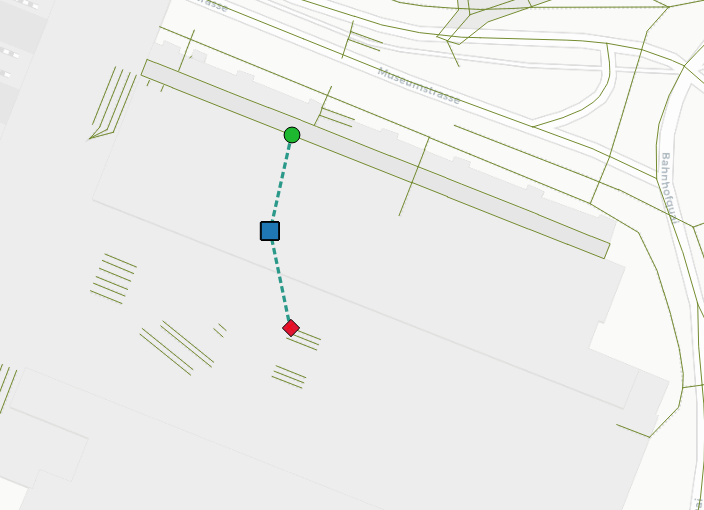
\includegraphics[width=1\linewidth]{projectdoc/img/snapping_comparison}
    \caption[Snapping der Haltestelle auf den Routing-Graphen]{Die Haltestelle (blaues Quadrat) wird mit dem einfachen Ansatz zur Rolltreppe "`gesnapped"' (Roter Diamant), während die Optimierung (Grüner Punkt) ein Ergebnis erzeugt, dass mit dem restlichen Routing-Netz verbunden ist.}
    \label{fig:snapping_comparison}
\end{figure}

Ein optimierter Ansatz nimmt nicht direkt den nächstliegenden Punkt auf dem Routing-Graphen, sondern prüft, ob dieser ermittelte Vertex auf einem isolierten Segment des Graphen liegt.
Dafür werden mit Hilfe der Routing-Engine alle Punkte gesucht, die von diesem Vertex aus in 200 Metern Fussweg erreichbar sind.
Wenn es einen Punkt gibt, der mindestens 150 Meter entfernt vom Startpunkt ist, wird dies als genügend bewertet, um den Startpunkt für die Erzeugung von \glspl{Isochrone} zu verwenden.
Wenn diese Bedingung nicht erfüllt ist, werden iterativ andere Vertices geprüft (sortiert nach der Distanz zur Haltestelle), bis ein passender Vertex gefunden wird.
Der Code dazu ist in Listing \ref{listing:snap_routing_graph} ersichtlich.

\begin{listing}[ht]
    \inputminted{sql}{projectdoc/listing/nearest_neighbor.sql}
    \caption{SQL Stored Procedure für das "`Snapping"' der Haltestelle auf den Routing-Graph}
    \label{listing:snap_routing_graph}
\end{listing}

Das Ergebnis für den Zürcher Hauptbahnhof ist in Abbildung~\ref{fig:snapping_comparison} zu sehen.
Dieser Startpunkt ist noch immer nicht optimal, da ein Fussgänger auch ein Ausgang auf der anderen Seite des Bahnhofes wählen könnte.
Für eine optimale Bestimmung müsste der Routing-Graph mit zusätzlichen Wegen ergänzt werden.
Fussgängerflächen könnten beispielsweise durch eine Vorverarbeitung durch \emph{PlazaRoute}~\cite{plaza_route} in den Routing-Graph integriert werden. Dabei werden zusätzliche Graph-Kanten eingefügt.

\subparagraph{Vorbereitung des Routing-Graphen}
Zum Zeitpunkt des Imports mit \emph{OSM2PO} besteht ein vollständiger Routing-Graph, auf dem bereits Routen berechnet werden können.
Für die Berechnung von \glspl{Isochrone} ist dieser Routing-Graph aber nicht geeignet, da jeder Strassenabschnitt von einer Verzweigung zur nächsten als eine einzige Kante abgebildet wird.
Werden nun \glspl{Isochrone} erstellt, beachtet der Algorithmus nur Vertices, die komplett in der definierten Zeit erreichbar sind.
Dadurch werden Strassen ausgeschlossen, die innerhalb der Zeit nur bis zu einem Teil der Strecke erreichbar sind.
Dies führt zu ungenauen \glspl{Isochrone}, wie in Abbildung \ref{fig:vergleich_segmentierung} ersichtlich ist.

Um diesen Effekt zu vermindern, wird vor der Berechnung der komplette Routing-Graph segmentiert.
Dazu werden alle Kanten in einzelne Segmente geteilt, die maximal 30 Meter lang sind.
Anschliessend muss die Topologie erneut berechnet werden, um die Verbindungen von Kanten und Vertices zu aktualisieren.
Die daraus resultiertenden \glspl{Isochrone} sind deutlich genauer und bilden ein realistischeres Einzugsgebiet ab (siehe Abbildung \ref{fig:vergleich_segmentierung}).

\begin{figure}[ht]
    \centering
    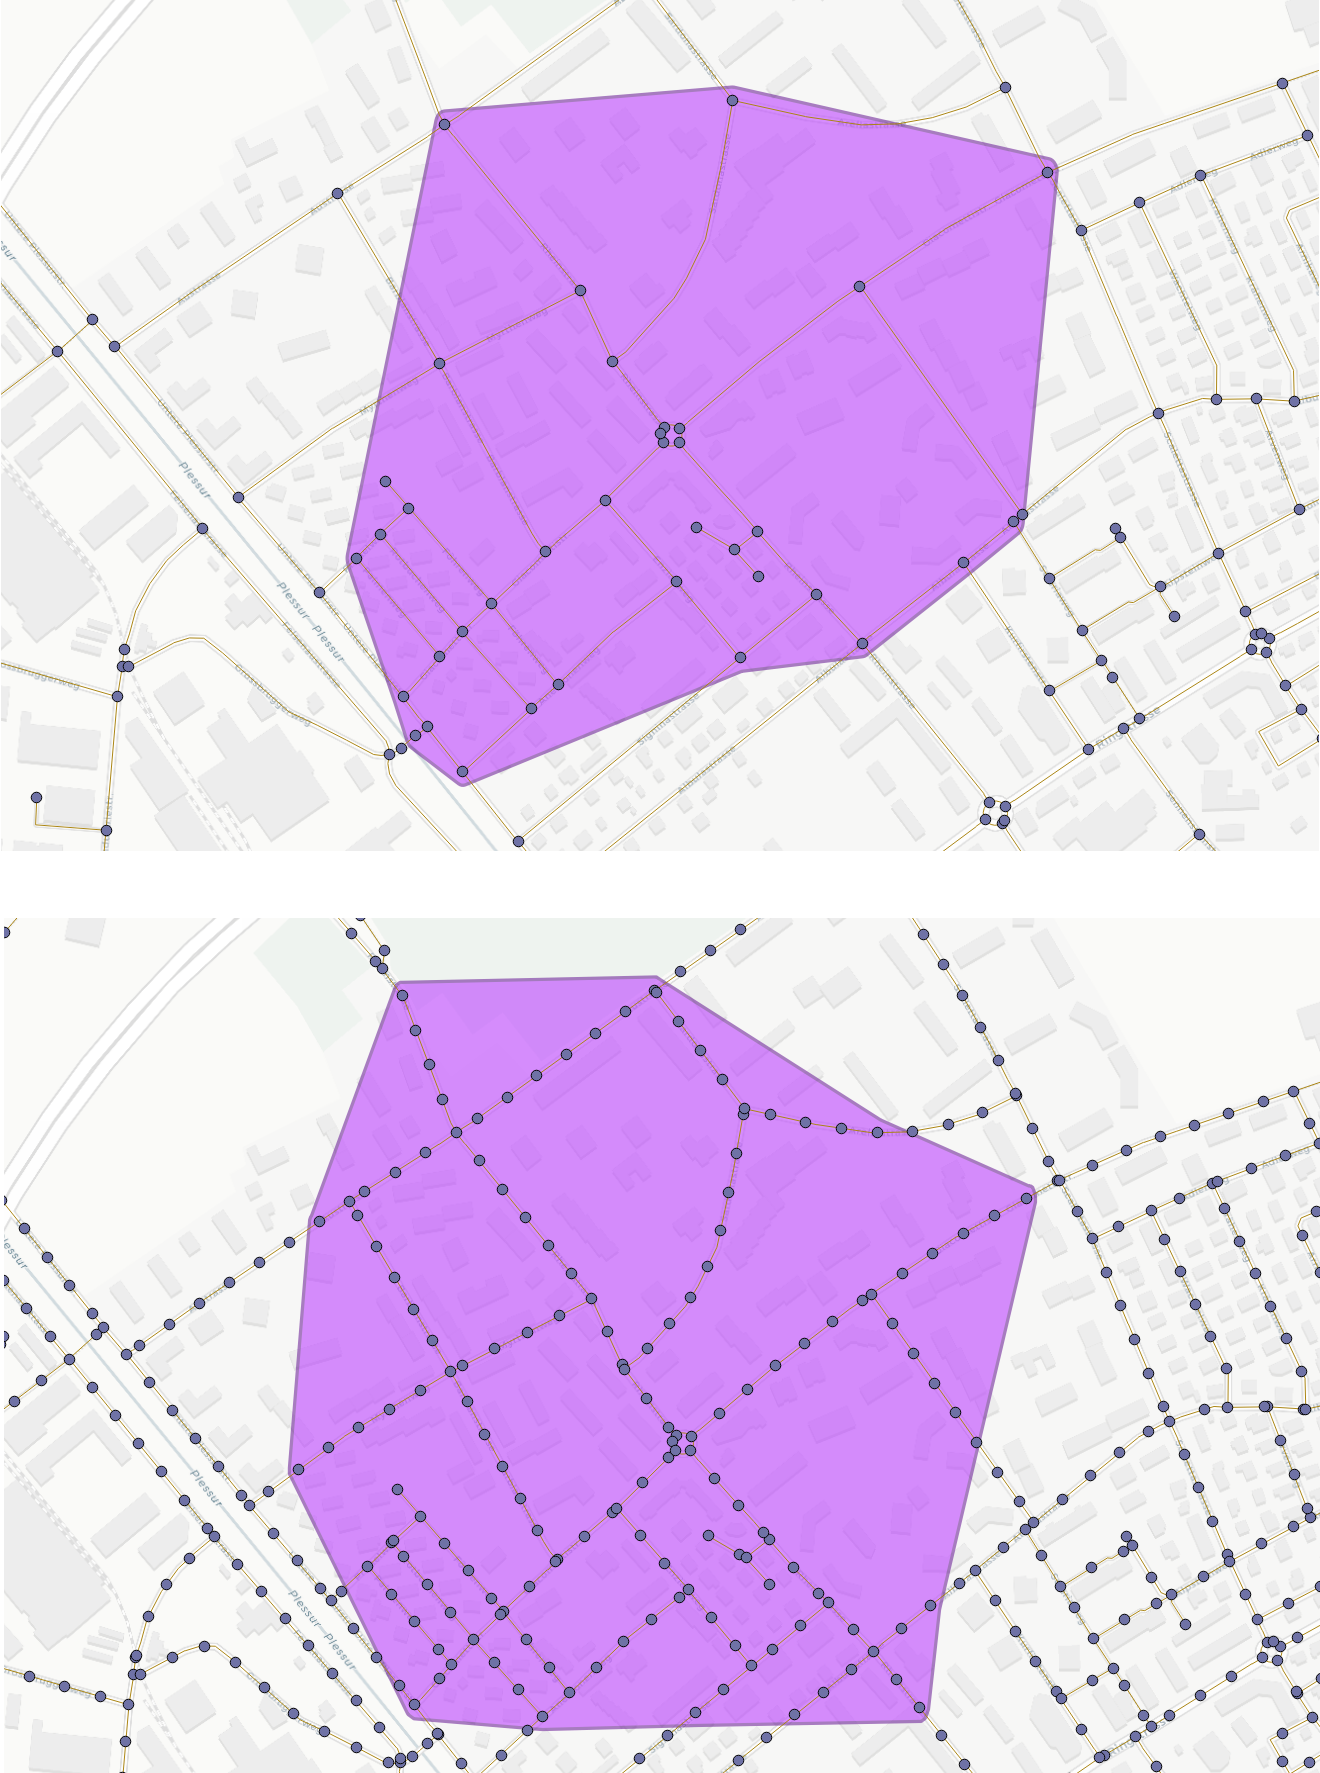
\includegraphics[width=0.5\linewidth]{projectdoc/img/vergleich_segmentierung}
    \caption[Vergleich von Isochronen bei regulärem und segmentiertem Routing-Graph]{Mit der Segmentierung des Routing-Graphen (unten) ergeben sich gegenüber des regulären Graphen (oben) höher aufgelöste Isochronen}
    \label{fig:vergleich_segmentierung}
\end{figure}

Als weiteren Schritt der Vorbereitung werden die Terrain-Daten in die Kosten der Kanten eingerechnet.
Dazu wird die Formel aus der Spezifikation für Leistungskilometer (siehe \ref{Berechnungsmethodik OeVGK18:Gehzeit zur Haltestelle}) verwendet.
Für jede Kante werden die Kosten in beide Richtungen berechnet, da Steigung und Gefälle unterschiedlich gewichtet werden.

\subparagraph{Berechnung der Isochronen}
In einem ersten Schritt wird ermittelt, welche \glspl{Isochrone} für die gegebene Haltestelle erzeugt werden müssen.
Dabei wird die Gehzeit mithilfe der konfigurierten Laufgeschwindigkeit in Meter umgerechnet, da die Kosten des Routing-Graphen ebenfalls in Meter abgebildet sind.

Anschliessend werden die \glspl{Isochrone} berechnet.
Dieser Algorithmus besteht aus zwei Teilen.
Als erstes werden mit dem Dijkstra-Algorithmus~\cite{dijkstra_algorithm} alle Vertices ermittelt, die von der Haltestelle aus in der festgelegten maximalen Laufdistanz im Routing-Graph erreichbar sind (siehe Listing \ref{listing:calc_isochrones_dijkstra}).
Die Richtung der Kanten wird dabei umgekehrt, da der Dijkstra-Algorithmus die Strecke ausgehend der Haltestelle berechnet.
Für unsere Zwecke ist es aber realistischer, den Laufweg zu berechnen, wenn man zur Haltestelle hin läuft.

\begin{listing}[ht]
    \inputminted{sql}{projectdoc/listing/calc_isochrones_dijkstra.sql}
    \caption[Dijkstra-Algorithmus zur Berechnung von Isochronen]{Mit einem Dijkstra-Algorithmus werden bis zur Maximaldistanz alle erreichbaren Vertices gesucht (Auszug)}
    \label{listing:calc_isochrones_dijkstra}
\end{listing}

Vorgängig werden mit einer Query alle Kanten gesucht, die sich in einem Radius von 1300 Metern der Haltestelle befinden (siehe Listing \ref{listing:calc_isochrones_preselection}).
Dies, weil keine Isochronen berechnet werden, die einen grösseren Radius als 1300 Meter einschliessen.
Dadurch verringert sich die Anzahl Kanten enorm, die pgRouting mit dem Dijkstra-Algorithmus abarbeiten muss.

\begin{listing}[ht]
    \inputminted{sql}{projectdoc/listing/calc_isochrones_preselection.sql}
    \caption[Vorselektion der Kanten für die Berechnung von Isochronen]{Mit einer effizienten Index-Suche werden alle Kanten in der Nähe der Haltestelle ermittelt (Auszug)}
    \label{listing:calc_isochrones_preselection}
\end{listing}

Im zweiten Schritt wird mit diesen Vertices eine Alpha Shape~\cite{alpha_shapes} erzeugt (siehe Listing \ref{listing:calc_isochrones_alpha_shape}). Dieser Algorithmus bildet das kleinst mögliche Polygon, wobei alle gefunden Vertices darin enthalten sein müssen.
Diese Alpha Shape stellt die \gls{Isochrone} dar.

\begin{listing}[ht]
    \inputminted{sql}{projectdoc/listing/calc_isochrones_alpha_shape.sql}
    \caption[Berechnung der Alpha Shape]{Mit den erreichbaren Vertices wird eine Alpha Shape erzeugt (Auszug)}
    \label{listing:calc_isochrones_alpha_shape}
\end{listing}

Der erste Schritt muss pro Haltestelle nur ein Mal für die grösste zu berechnende Distanz durchgeführt werden, für die Erzeugung der \glspl{Isochrone} für kürzere Distanzen wird das Ergebnis des Dijkstra-Algorithmus gefiltert und nur die Vertices beachtet, die innerhalb dieser Distanz von der Haltestelle erreichbar sind.
Auf die einzelnen \glspl{Isochrone} wird ein zusätzlicher Buffer angewendet, um die scharfen Ecken etwas abzurunden.
Dadurch wird bewusst etwas Unschärfe hinzugefügt, um nicht die Illusion zu erwecken, dass die \gls{Isochrone} das Einzugsgebiet exakt abbildet, sondern nur eine Approximation dessen darstellt.

\paragraph{Ausgabe des Ergebnisses}~\\
Nach der Berechnung der \acs{ÖV}-Güteklassen liegt für jede Haltestelle, die mindestens eine Basiserschliessung hat, ein oder mehrere \glspl{Isochrone} vor.
Diese gilt es nun im GeoJSON Format auszugeben.
Dabei wird für jeden der unterschiedlichen Stichtage eine separate Datei erstellt.

Für jede \gls{Isochrone} wird ein GeoJSON-Feature erstellt, wobei die \acs{ÖV}-Güteklasse und die \emph{uic\_ref} der Haltestelle als zusätzliche Attribute mitgegeben werden.
Anschliessend werden alle Features sortiert nach \acs{ÖV}-Güteklassen, wobei die tieferen Klassen zuerst eingefügt werden.
Dies hat später für die Visualisierung eine Auswirkung.
Weil die \glspl{Isochrone} der höheren Klassen diejenigen der tieferen überlagern, sollten bei der Visualisierung die tieferen Klassen zuerst gerendert werden.
Durch die Reihenfolge wird dies bereits in diesem Schritt sichergestellt.

Zusätzlich zu den \acs{ÖV}-Güteklassen wird eine GeoJSON-Datei mit den Punkten aller Haltestellen erstellt, um sie später mit der Web-Applikation auf der Karte anzeigen zu können.
Ebenfalls wird eine JSON-Datei geschrieben mit Metadaten zu den Parametern der einzelnen Stichtage, die für die Berechnung verwendet wurden.
Mit dieser JSON-Datei wird dem Backend ebenfalls mitgeteilt, welche Stichtage angeboten werden können.

\subsection{Backend}
\label{Implementation:Backend}

In diesem Abschnitt wird die Implementation des Containers \nameref{container:Backend} erläutert.
Primäres Ziel der Komponente ist es, Nutzer Informationen über verfügbare \acs{ÖV}-Güteklasse bereitzustellen.
Es handelt sich dabei um eine schlanke Flask-Applikation~\cite{flask} mit sehr geringer Logik.

Das Backend wird beim Starten initialisiert.
Dabei wird eine generierte Metadaten-Datei des Container \nameref{container:generator} eingelesen.
Genauer Sinn und Zweck dieser Datei ist im Abschnitt \ref{layer:output} beschrieben.
Diese Datei beinhaltet Informationen, welche \acs{ÖV}-Güteklassen verfügbar sind.
Dadurch kann die Web-App entscheiden, welche \acs{ÖV}-Güteklassen der Benutzer auswählen kann und wie diese vom Container \nameref{container:Tile-Server} bezogen werden können.

Diese Informationen werden über ein Web-\ac{API} exponiert.
Diese besteht aus \acl{REST}-Services.
Die verfügbaren Services sind in der Tabelle \ref{table:Wep-API} beschrieben.
Im Bezug auf das Maturity Model~\cite{maturity_model} von Leonard Richardson befinden wir uns auf Level 2.

Mithilfe von Flasgger~\cite{flasgger} wird eine \ac{OAS}~\cite{open-api-specificaiton} erstellt.
Dies hat den Vorteil, dass das \ac{API} sauber dokumentiert ist und Clients der \ac{API} in unterschiedlichen Sprachen generiert werden können.

Das konkrete Web-\ac{API}, welches das Backend exponiert, kann mit ReDoc (OpenAPI/Swagger-generated API Reference Documentation)~\cite{oevgk18-backend-api-spec} oder mit dem klassischen Swagger UI~\cite{oevgk18-backend-api-swaggerui} betrachtet werden.

\subsection{Tile-Server}
\label{Implementation:Tile-Server}

Als Tile-Server bietet sich TileServer GL~\cite{tile-server-gl} an.
Wie die GeoJSON in ein vom Tile-Server unterstütztes Format gelangen, ist im Abschnitt \ref{Implementation:Tile-Converter} beschrieben.

Der Tile-Converter ist als Docker-Container verfügbar.
Dieser wird im Kapitel \ref{Infrastruktur:Deployment} genauer beschrieben.


\subsubsection{Tile-Converter}
\label{Implementation:Tile-Converter}

Der Container \nameref{container:generator} generiert die \acs{ÖV}-Güteklassen aktuell im GeoJSON-Format.
Damit der Tile-Server Vector Tiles ausliefern kann, müssen die \acs{ÖV}-Güteklassen in ein entsprechendes Format umgewandelt werden.
Der oben erwähnte Tile-Server nutzt MBTiles~\cite{mbtiles}.
Dabei handelt es sich um eine Spezifikation von Mapbox, um beliebige gekachelte Karten-Daten zu speichern.
Dieses Format ist extrem effizient für Transfers, was in unserer Problemdomain relevant ist.
Für die Konvertierung bietet sich das Tool \emph{tippecanoe}~\cite{tippecanoe}, ebenfalls von Mapbox, an.
Dieses erlaubt die Konvertierung von verschiedenen Dateiformaten, so auch GeoJSON in MBTiles und die Konfiguration der zu generierenden Vector Tilesets.

Die Indirektion über das GeoJSON-Format ist bewusst.
Die ÖV-Güteklassen können als GeoJSON breiter verwendet werden, etwa in QGIS.
Das MBTiles ist speziell auf Vector Tilesets ausgelegt, was bei uns nicht der Hauptfokus ist.

Der Tile-Converter ist als Docker-Container verfügbar.
Dieser wird im Kapitel \ref{Infrastruktur:Deployment} genauer beschrieben.

\subsection{Web-App}
\label{Implementation:Web-App}

In einer Evaluation, welche im Kapitel \ref{Analyse:Evaluation Frontend-Framework} beschrieben ist, wurde entschieden, dass der Fokus auf React~\cite{react} gelegt wird.
Die Web-App wurde dementsprechend mit React entwickelt.
Grafisch wurde das Frontend aufgrund der \nameref{appendix:wireframes} umgesetzt.
Ein Auszug ist in Abbildung \ref{fig:Web_App} ersichtlich.

\begin{figure}[ht]
    \centering
    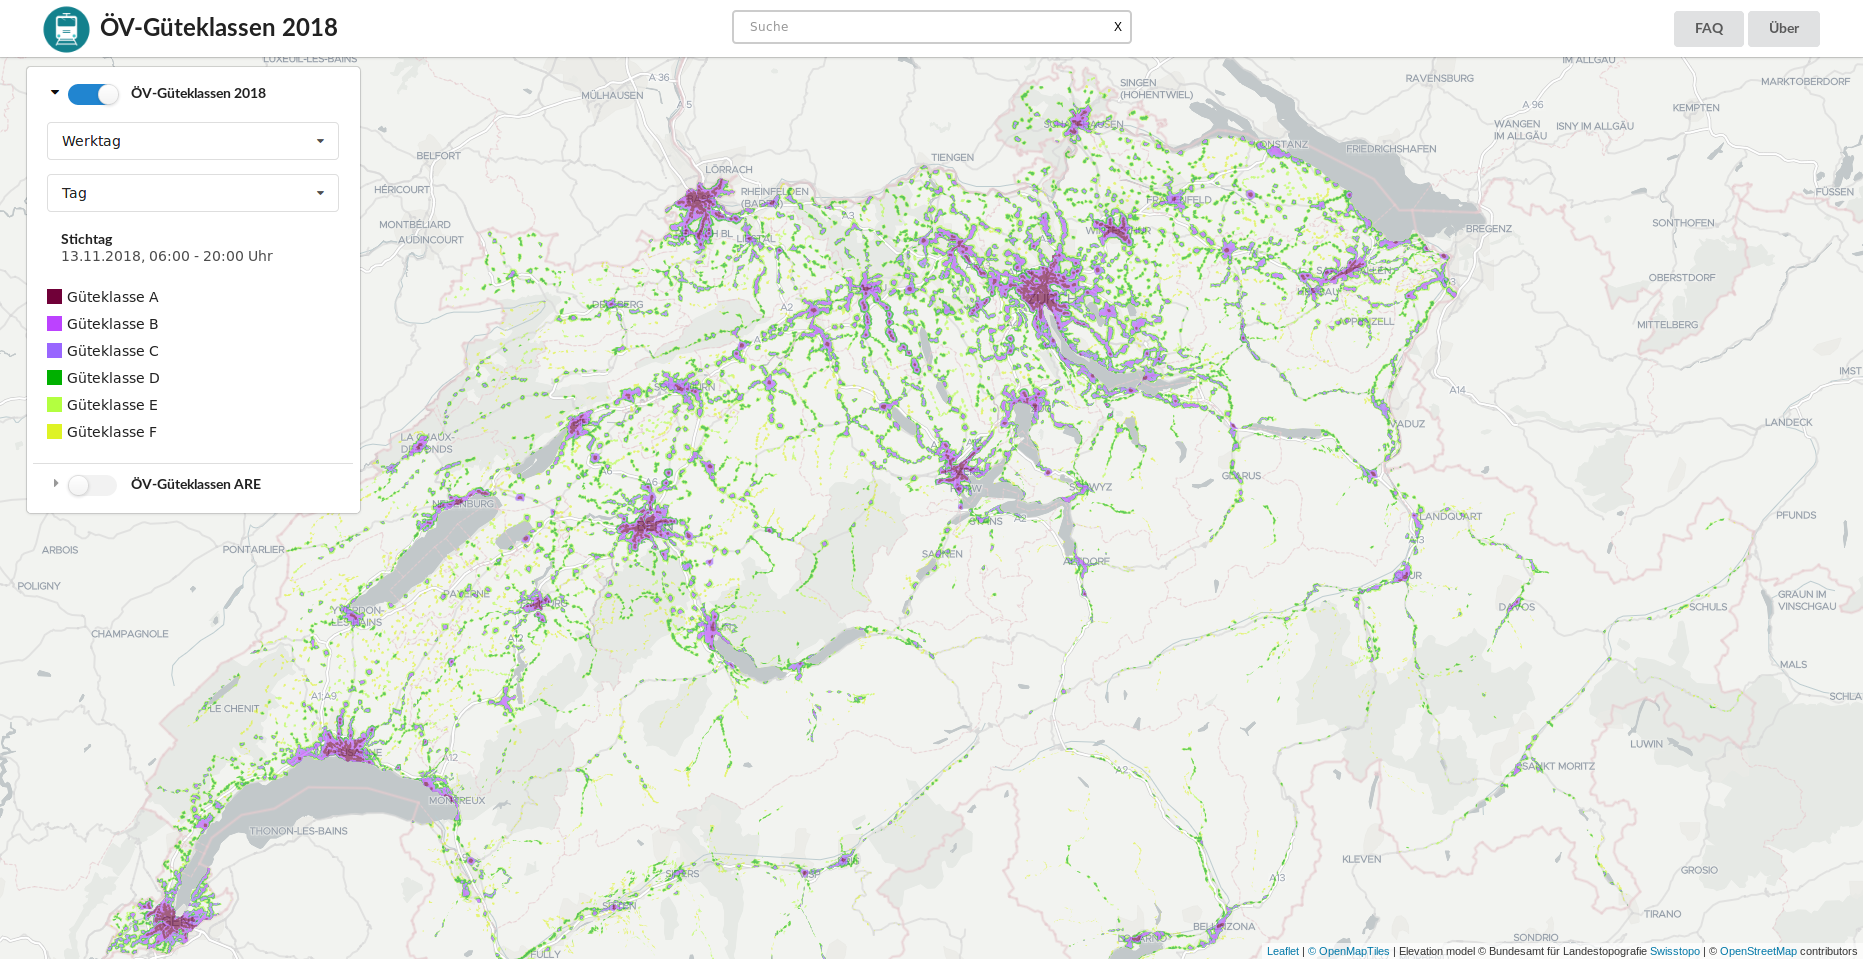
\includegraphics[width=1.0\linewidth]{projectdoc/img/screenshot-webapp.png}
    \caption[Web-App]{Web-App}
    \label{fig:Web_App}
\end{figure}

Zur Übersicht sind die React-Komponenten in einer Baumstruktur in Abbildung \ref{fig:Web_App_Component} aufgeschlüsselt.
Dabei handelt es sich im engeren Sinn nicht um ein klassisches UML-Komponenten-Diagramm.
Die Verantwortlichkeiten werden nachfolgend kurz beschrieben.

\begin{figure}[H]
    \centering
    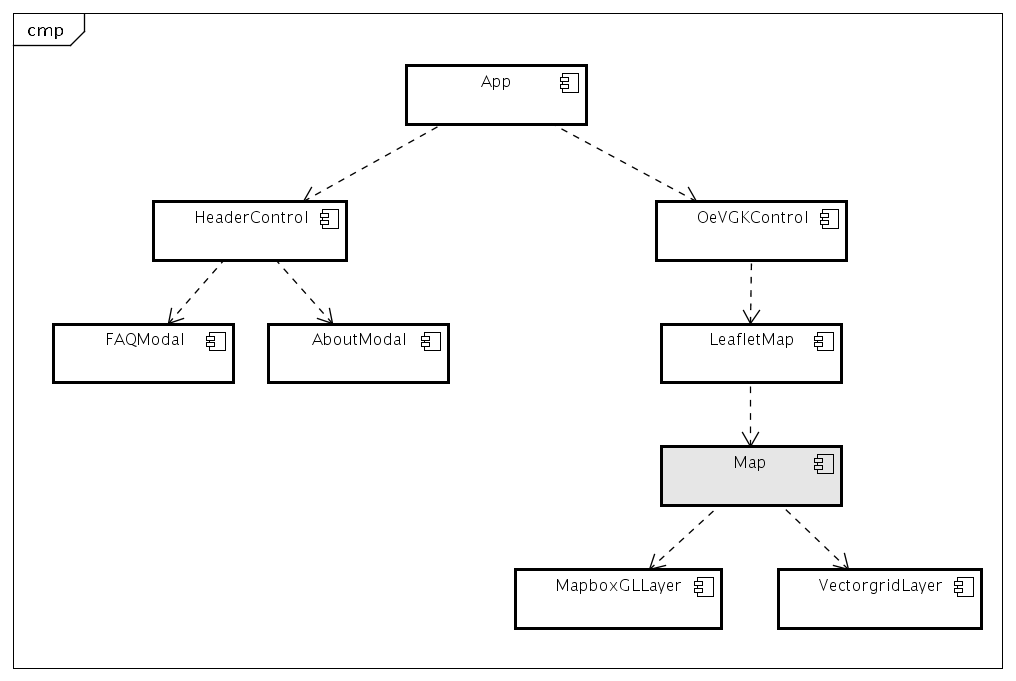
\includegraphics[width=1.0\linewidth]{projectdoc/img/Web-App_Component.png}
    \caption[Web-App React Komponente Übersicht]{Web-App React Component Übersicht (grau: externe Komponente)}
    \label{fig:Web_App_Component}
\end{figure}
 
\paragraph{App}
Der zentrale Einstieg der React-Applikation ist die \emph{App}-Komponente.

\paragraph{HeaderControl}
Der ganze Header wird über den \emph{HeaderControl} verwaltet, welche aus zwei Modals (=Dialogen) besteht, die geöffnet werden können.
Zur einfachen Bedienung ist ebenfalls ein \gls{Geocoding} als Suchfunktion eingebunden.

\paragraph{OeVGKControl}
Interessant ist die Haupt-Komponente \emph{OeVGKControl}, welche die Benutzereingaben und die Karte kontrolliert.
Diese Komponente nutzt das Web-\acs{API} vom Backend.
Der Ablauf ist stark vereinfacht in Abbildung \ref{fig:Web-App_Sequence} sichtbar.
Beim Mounten dieser Komponente werden vom Backend die verfügbaren Stichtage angefragt (Schritt 1 und 2).
Anschliessend werden für einen Stichtag die zugehörigen Zeitintervalle geladen (Schritt 3 und 4).
Mit diesen beiden Informationen werden vom Tile-Server dann die gewünschten \acs{ÖV}-Güteklassen geladen (Schritt 7).
Wählt der User einen neuen Stichtag oder Zeitintervall, wiederholt sich der Ablauf.

\begin{figure}[ht]
    \centering
    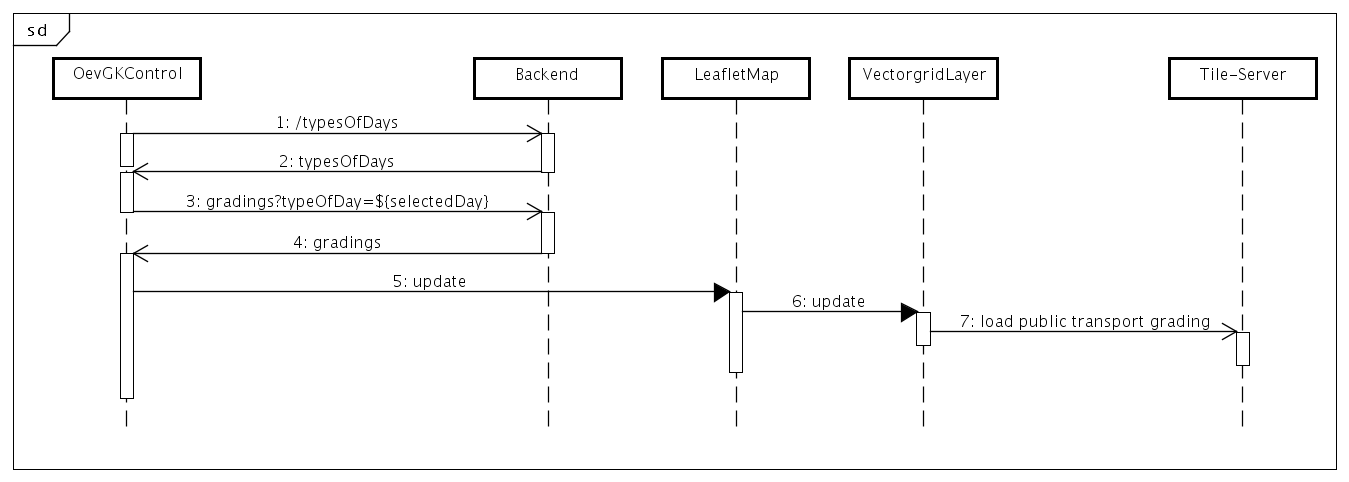
\includegraphics[width=1.0\linewidth]{projectdoc/img/Web-App_Sequence.png}
    \caption[Auszug Zusammenspiel React Components]{Auszug Zusammenspiel React Components}
    \label{fig:Web-App_Sequence}
\end{figure}

Es sei angemerkt, dass auf dem Tile-Server für einen Satz von \acs{ÖV}-Güteklassen nicht nur einmal zugegriffen wird, wie man aufgrund der Sequenz annehmen könnte.
Der Vorteil der Vector Tiles und dem damit verbundenen Tile-Server liegt darin, dass gerade nur die Tiles geladen werden, welche benötigt werden. Verändert man Auszug und Zoomstufe, löst man somit Zugriffe auf den Tile-Server aus.

\paragraph{LeafletMap}
\emph{LeafletMap} ist für die Darstellung der Karte verantwortlich.
Dabei wird die Komponente \emph{Map} von react-leaflet~\cite{react-leaflet} verwendet.
Mithilfe von Mapbox GL JS (MapboxGLLayer)~\cite{mapbox_gl_leaflet} kann die Basiskarte ebenfalls mit Vector Tiles abgebildet werden, was standardmässig von Leaflet nicht unterstützt wird.

\paragraph{VectorgridLayer}
Die Kartendaten, welche über die Basiskarte gerendert werden, werden mit der Komponente \emph{VectorgridLayer} verwaltet.
So existiert jeweils ein Layer für die \acs{ÖV}-Güteklassen 2018, für die \acs{ÖV}-Güteklassen des \acl{ARE} und eine für die ÖV-Haltestellen.
Somit werden alle Kartendaten mit Vector Tiles abgebildet.
Alle diese Layer sind in Abbildung \ref{fig:Vector-Grid-Layers} ersichtlich.

\begin{figure}[ht]
    \centering
    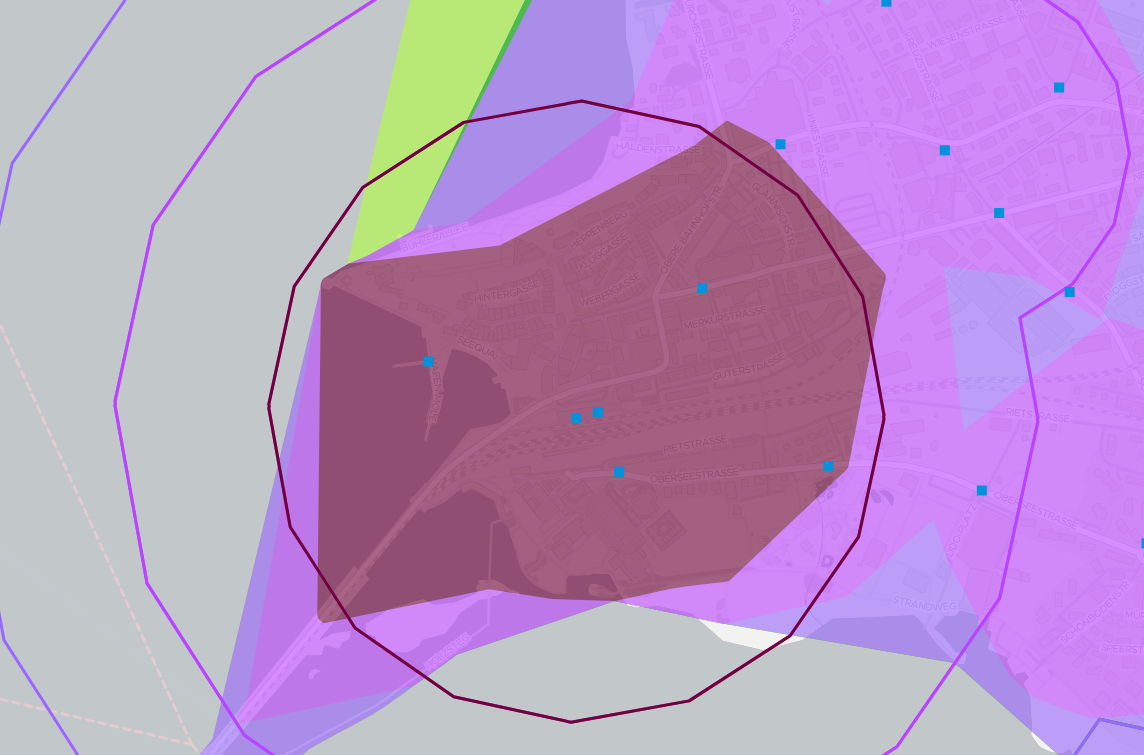
\includegraphics[width=0.6\linewidth]{projectdoc/img/vectorgrid_layers.png}
    \caption[Vector-Grid Layers]{Vector-Grid Layers}
    \label{fig:Vector-Grid-Layers}
\end{figure}

Beim Layer, welcher die ÖV-Haltestellen anzeigt, ist der Vorteil der Vector Tiles stark sichtbar.
So wurden diese Vector Tiles so konfiguriert, dass sie erst ab einer gewissen Zoomstufe angezeigt werden. In der Abbildung \ref{fig:zoom-level-comparison} sieht man den Unterschied zwischen Zoomstufe 13 (links) und 14 (rechts).
Dadurch müssen auf einer tieferen Zoomstufe weniger grosse Vector Tiles geladen werden und der Fokus bleibt auf den \acs{ÖV}-Güteklassen.

\begin{figure}[ht]
    \centering
    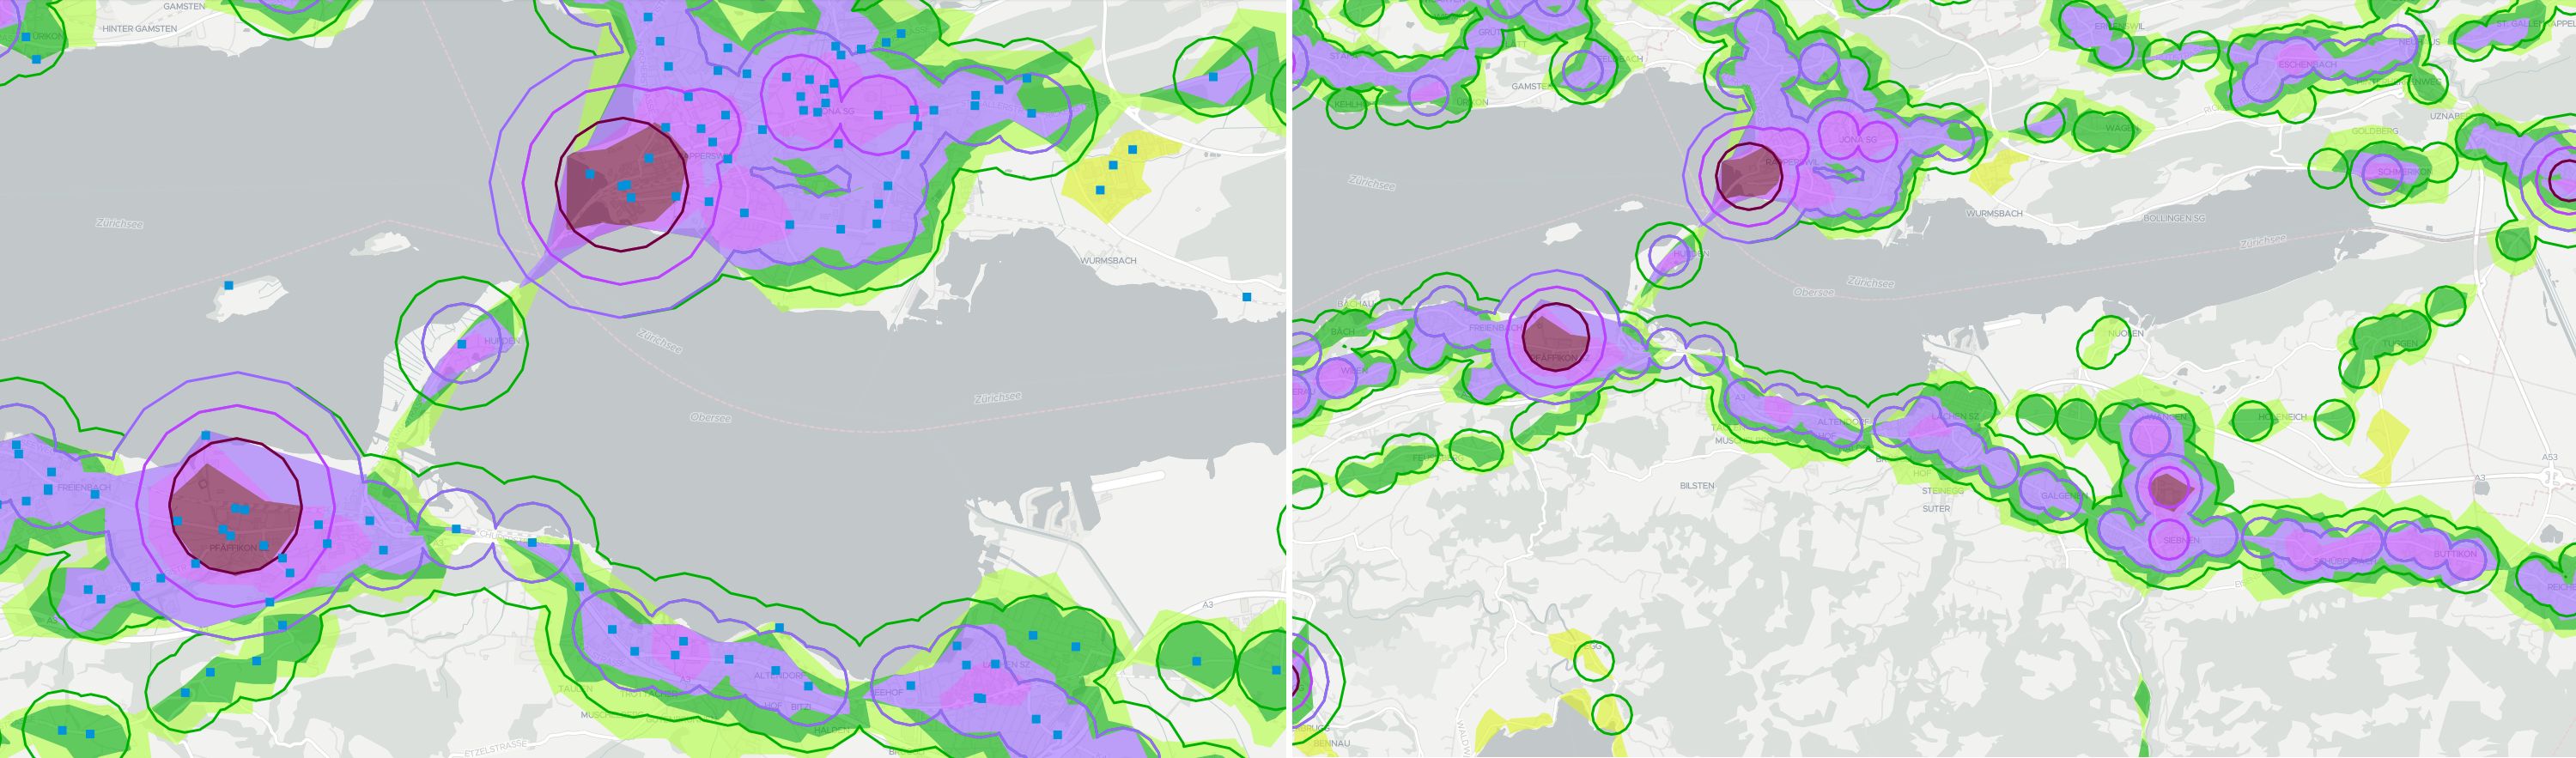
\includegraphics[width=1.0\linewidth]{projectdoc/img/zoom-level-comparison.png}
    \caption[Vergleich Zoom-Stufe ÖV-Haltestelle Layer]{Vergleich Zoomstufe ÖV-Haltestelle Layer: Zoomstufe 13 (links) und 14 (rechts)}
    \label{fig:zoom-level-comparison}
\end{figure}


\subsubsection{Wechsel von Mapbox GL auf Leaflet}

In einer Analyse wurden die beiden Frontend-Frameworks Vue.js und React evaluiert (siehe Kapitel~\ref{Analyse:Evaluation Frontend-Framework}).
Die Unterstützung von Mapbox GL JS~\cite{mapbox_gl_js} war das ausschlagende Kriterium für den Entscheid zugunsten von React.
Der Grund für den Einsatz von Mapbox GL JS gegenüber Leaflet~\cite{leaflet} war die gute Unterstützung von Vector Tiles.
Trotz alldem hat sich während der Entwicklung gezeigt, dass der Wechsel zu Leaflet praktisch unausweichlich ist.
Im Folgenden ist dieser Schritt begründet.

Der ausschlaggebende Nachteil von Mapbox GL JS zeigte sich bei der Integration der \acs{ÖV}-Güteklassen, um sie auf der Webkarte anzeigen zu können.
Wenn sich mehrere Haltestellen nah beieinander befinden, überschneiden sich ihre \glspl{Isochrone}.
Da wir hinter den Geometrien der \acs{ÖV}-Güteklassen auch die Basiskarte im Hintergrund anzeigen möchten, muss die Deckkraft der Geometrien entsprechend verringert werden.
Mapbox GL JS unterstützt die Einstellung der Deckkraft aber ausschliesslich auf Feature-Ebene, sprich auf einzelnen Geometrien.
Bei sich überlagernden Features entsteht damit der Effekt, dass die Farben sich mischen und einander verstärken (siehe Abbildung~\ref{fig:problem_overlapping_isochrones}).
Dies ist irreführend, da ein Gebiet mit zum Beispiel Güteklasse A durchgehend gleich kategorisiert werden soll, egal von wie vielen verschiedenen Haltestellen mit der gleichen Güteklasse das Gebiet erschlossen wird.

\begin{figure}[ht]
    \centering
    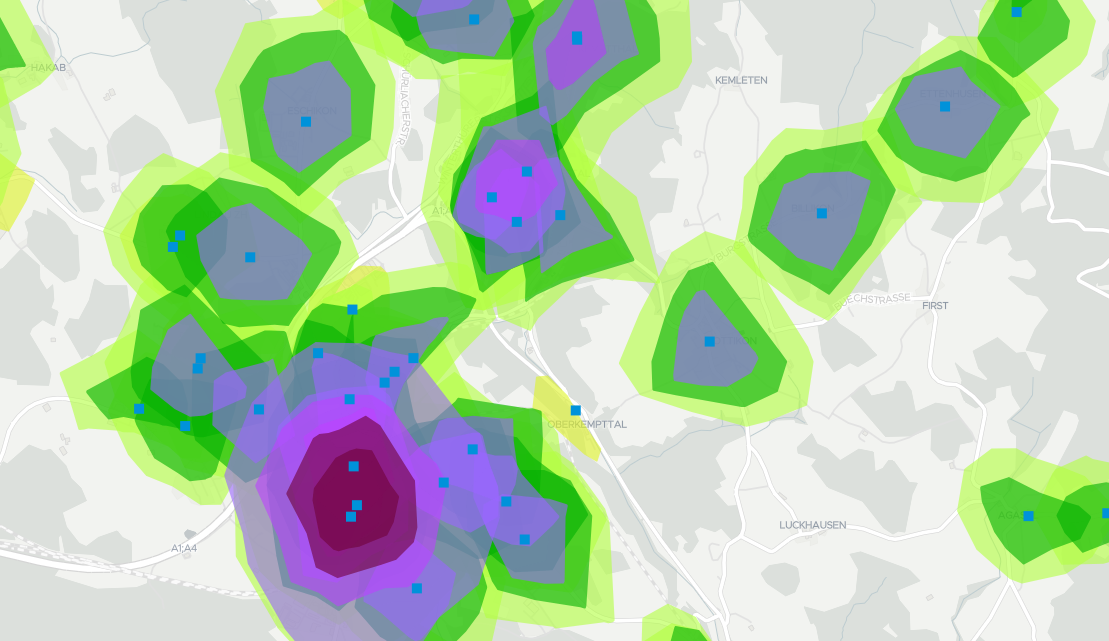
\includegraphics[width=0.8\linewidth]{projectdoc/img/problem_overlapping_isochrones}
    \caption[Problematik von sich überlappenden Geometrien mit gleicher Deckkraft]{Überlappende Geometrien mit gleicher Deckkraft ergeben gemischte und irreführende Farbflächen}
    \label{fig:problem_overlapping_isochrones}
\end{figure}

Für die Lösung dieses Problems gibt es zwei Ansätze:

\begin{enumerate}
    \item Die Deckkraft der einzelnen Geometrien auf 100\% setzen und dabei die Deckkraft des kompletten Layers verringern
    \item Die Geometrien voneinander ausschneiden, so dass keine Überlagerungen mehr existieren
\end{enumerate}

Der erste Ansatz ist mit Mapbox GL JS momentan nicht möglich.
Die Unterstützung dafür wird aktuell auf Github diskutiert und steht noch offen~\cite{mapbox_layer_opacity}.
Der zweite Ansatz wurde während der Entwicklung implementiert.
Da alle Geometrien von allen anderen ausgeschnitten werden, ist dies eine komplexe Operation in der Grössenordnung $\mathcal{O}(n^2)$.
Mit einem R-Tree-Index kann diesem Problem entgegen gesteuert werden.
Es entstanden ausserdem Probleme mit der Topologie der ausgeschnittenen Geometrien sowie Render-Fehler im Browser.

Diese Problematiken haben uns dazu bewegt, von Mapbox GL JS auf Leaflet umzusteigen.
Die erste Option, die Verringerung der Deckkraft auf dem kompletten Layer, ist dort kein Problem.
Damit wurde auch das Ausschneiden der einzelnen Geometrien überflüssig.

\paragraph{Vector Tiles mit Leaflet}~\\
Der Wechsel zu Leaflet bedeutet auch, dass Vector Tiles nicht mehr nativ unterstützt werden.
Allerdings gibt es mit \emph{Leaflet.VectorGrid}~\cite{leaflet_vector_grid} eine Erweiterung, die genau dies erlaubt.
Dafür gibt es zwar keine vorgefertigten React-Komponenten, mit etwas Handarbeit können diese aber leicht selbst erstellt werden.

Ein Spezialfall ist das Einbinden der Basiskarte, die von OpenMapTiles~\cite{openmaptiles} bezogen wird.
Diese wird von \emph{VectorGrid} nicht unterstützt.
Es gibt aber wiederum von Mapbox selbst eine Library, um Mapbox GL JS in einer Leaflet-Karte einzubinden~\cite{mapbox_gl_leaflet}.
Somit haben wir schlussendlich einen Hybrid aus Mapbox GL JS und Leaflet, wobei Mapbox GL JS nur für die Basiskarte verwendet wird, wo die oben genannten Probleme mit der Deckkraft nicht relevant sind.
